\documentclass[10pt,a4paper,landscape]{article}
\usepackage[latin1]{inputenc}
\usepackage{amsmath}
\usepackage{amsfonts}
\usepackage{amssymb}
\usepackage{graphicx}
\usepackage[left=0.00cm, right=0.00cm, top=0.00cm, bottom=0.00cm]{geometry}
\usepackage{multirow}
\usepackage{array}
\usepackage{tikz}
\usepackage{collcell}
\usepackage{calc}
%\usepackage{fontspec}
\begin{document}
\setlength{\tabcolsep}{0pt}
\renewcommand{\arraystretch}{0}
\setlength{\parindent}{0pt}
\setlength{\parskip}{0pt}
\renewcommand{\familydefault}{\sfdefault}
\pagestyle{empty}  % no page number

% the tikz wrapper command that formats each label
% contains some stuff that you may not want - just
% for illustrating that it is easy enough in case you do
\newcommand{\CutMarkCell}[1]{%
	\tikz{%
		\node[
			align=center,                   % center text
			outer sep=0mm,                  % no padding on the outside
			inner sep=0mm,                  % no inner padding
			minimum height=15mm,            % scale height
			text width=10mm,    		 	% text width
			rounded corners=2pt] {#1}}}     % round corners with given radius

\newcommand{\TopBottomCell}[1]{%
\vspace*{5mm}
	\tikz{%
		\node[
			align=center,                   % center text
			outer sep=0mm,                  % no padding on the outside
			inner sep=0mm,                  % no inner padding
			% minimum height=7.5mm,            % scale height
			%minimum height=1mm
			text width=10mm,    		 	% text width
			rounded corners=2pt] {#1}}}     % round corners with given radius

\newcommand{\PictureCell}[1]{%
	\tikz{%
		\node[
			align=center,                   % center text
			outer sep=0mm,                  % no padding on the outside
			inner sep=0mm,                  % no inner padding
			minimum height=65mm,            % scale height
			text width=80mm,    		 	% text width
			rounded corners=2pt] {#1}}}     % round corners with given radius

\newcommand{\BetweenCell}[1]{%
	\tikz{%
		\node[
			align=center,                   % center text
			outer sep=0mm,                  % no padding on the outside
			inner sep=0mm,                  % no inner padding
			minimum height=7.5mm,            % scale height
			text width=10mm,    		 	% text width
			rounded corners=2pt] {#1}}}     % round corners with given radius

\newcommand{\AprilTagCell}[1]{%
	\tikz{%
		\node[
			align=center,                   % center text
			outer sep=0mm,                  % no padding on the outside
			inner sep=0mm,                  % no inner padding
			minimum height=65mm,            % scale height
			text width=80mm,    		 	% text width
			rounded corners=2pt] {#1}}}     % round corners with given radius

\newcommand{\PictureDistanceCell}[1]{%
	\tikz{%
		\node[
		align=center,                   % center text
		outer sep=0mm,                  % no padding on the outside
		inner sep=0mm,                  % no inner padding
		minimum height=65mm,            % scale height
		text width=10mm,    		 	% text width
		rounded corners=2pt] {#1}}}     % round corners with given radius

\newcommand{\AprilTagPicture}[1]{%parameter 1: page number=ApriltagID+1
	\centering
	\includegraphics[
		page=#1,%page number: Note: ApriltagID+1=page number!
		width=65mm,
		height=65mm,
		keepaspectratio,
		clip,trim=21.5mm 53.2mm 21.5mm 53.3mm,
		]{../data/raw_apriltags/tag36h11}
}

\newcommand{\Picture}[1]{%parameter 1: page number=ApriltagID+1
	\centering
	\includegraphics[
		width=65mm,
		height=65mm,
		keepaspectratio,
		]{../data/sign_pictures/#1}
}

\newcommand{\TrafficSignPicture}[1]{%parameter 1:picture name
	\centering
	\includegraphics[
		width=65mm,
		height=65mm,
		keepaspectratio,
		]{../data/sign_pictures/#1}
}


\newcommand{\DateBack}{
	\centering
	\rotatebox[origin=c]{180}{\small{\today}}
	\vspace{60mm}
}

%%%%%%%%%%%%%%%%%%%%%%%%%%%%%%%%%%%%%%%%%%%%%%%%%%%%%%%%%%%%%%%%%%
%% start python generated latex script
